\chapter{Image Registration based Motion Estimation}
\label{hammer}


For any image based diagnosis algorithm it is important that we are able to robustly extract features that characterize the pathology and use these to be able to classify the subjects. The difference between feature extraction and classification is somewhat arbitrary: An ideal feature extractor would yield a representation that makes the job of the classifier trivial; conversely, an ideal classifier would not need the help of a sophisticated feature extractor. However, feature extractors play another important role which is particularly important in our case, that of dimension reduction. 

Most of the work done under CAD has focused on pathologies that can be characterized by structural changes, like tumors. The only case where diagnosis of pathologies has utilized functional information invloves functional imaging modalities like fMRI or PET. Structural information, albeit important, is not sufficient to characterize cardiomyopathies. Cardiomyopathies present themselves in different forms, both by structural changes like plaque formation, fat deposits, etc., and also functional changes like variations in ventricular wall motion, ejection fraction, and perfusion. Both of these need to be extracted from the image before accurate diagnosis can be done. A lot of work has been done in feature extractors for structural characterizations of disease. Work has been done on extracting image features like intensities and gradients \cite{intgrad}, moments \cite{hammer}\cite{moments}, Gabor features \cite{manju96}\cite{anant} and local frequency representations \cite{locfreq}. The problem with cardiomyopathies is that not all of them can be characterized by structural changes. Function at rest may be abnormal as a result of one of the spectrum of ischaemic heart diseases (ischaemia, infarction, hibernation) or of cardiomyopathy from other causes. During stress testing, new or worsening wall motion abnormalities are indicative of functionally significant coronary artery stenosis \cite{stenoses}. In addition, wall motion imaging to detect regional contractile reserve is an accurate measure of myocardial viability, and the results can help guide coronary revascularization therapy. Identifying changes in the myocardium based on both structural and functional changes makes the system more robust. Of course quantization of the myocardial wall motion represents a challenge in itself.

\section{Using MR Cine Sequences for Structural and Functional Characterization}
\label{sec:modality}

Since the ultimate goal is to be able to classify patient scans in order to diagnose cardiomyopathies, the following factors need to be considered for the choice of imaging modality.
\begin{itemize}
\item CAD applications are supposed to aid physicians during diagnosis and not really work independently. Therefore the modality being used by the CAD program should be convenient for the physician to use for diagnosis. In a typical setting the CAD program will filter our most of the patients scanned. The physician reevaluates these patients and removes the false positives from the filtered list. If the physician is not able to diagnose using the same images as that used by the CAD program then an additional set of images will need to be acquired for the physician to confirm the diagnosis  
\item The modality should be capable of providing both structural and functional information about the myocardium. This means that the modality should be able to provide 4D datasets. 
\item It is also preferable that we have a large enough database of available scans for normal and pathological cases so that we can train our classifier. It would be very difficult and expensive to acquire new datasets for different kinds of patients. This suggests the use of MR Cine sequences as it is very routine to acquire these for patients with most cardiomyopathies.
\item Since patients need to be scanned on a regular basis, the scan modality should be simple and patient discomfort and trauma should be minimal. This rules out modalities requiring intervention. This also implies minimizing the time spent inside the scanner by the patient and also the number of breathholds required for the scan.
\end{itemize} 

\begin{figure}
     \centering
     \subfigure[MR Cine]{
          \label{fig:mrcine}
          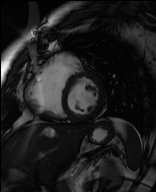
\includegraphics[width=.31\textwidth]{images/mr}}
     %%\hspace{.05in}
     \subfigure[MR Tagged]{
          \label{fig:mrtag}
          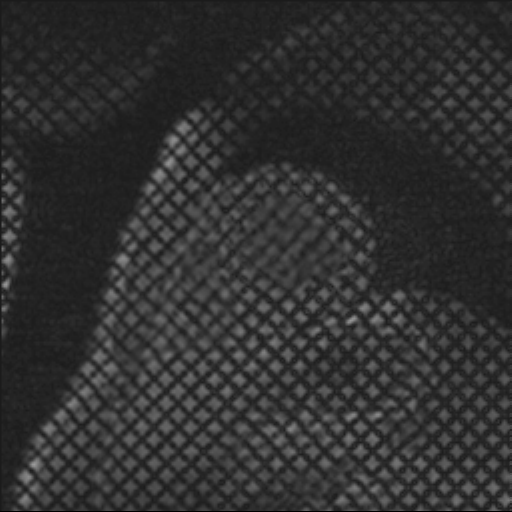
\includegraphics[width=.31\textwidth]{images/mr_tag}}
     %%\hspace{.05in}
     \subfigure[MR Phase Contrast]{
           \label{fig:mrphase}
           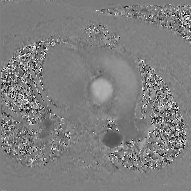
\includegraphics[width=.31\textwidth]{images/phase}}
     \caption{Different types of MR images}
     \label{fig:mrtypes}
\end{figure}

Most clinical modalities used to image myocardial function evaluate passive wall motion (ventriculography) or wall thickening (echocardiography, gated single-photon emission computed tomography, or cine MR imaging). MR imaging also allows quantitative measurement of regional intramyocardial motion and, subsequently, strain, which can be more sensitive to wall motion abnormalities than is wall thickening. The two most widely used MR imaging methods for the quantification of intramyocardial wall motion are myocardial tagging \cite{mrtag} and phase contrast imaging \cite{mrphase}. Each technique has advantages and disadvantages, which shall now be described.

MR Tagging was developed to provide non-invasive virtual markers inside the myocardium, which deform with myocardial motion \cite{mrtag}. MR imaging and especially tagged MR are currently the reference modalities to estimate dense cardiac displacement fields with high spatial resolution. The deformation fields, as well as the derived motion parameters such as myocardial strain can be determined with accuracy \cite{Shi99}\cite{mrtag1}\cite{chenBook}. The primary disadvantage of tagging is the reduced spatial resolution of strain relative to the image spatial resolution. In tagging, after the displaced tag lines are detected \cite{guttman94}, the displacement field can be estimated and intramyocardial strain can be computed in a variety of ways \cite{mrtag}. With this approach, although strain may be interpolated to any desired spatial resolution, the fundamental spatial resolution of strain is nominally determined by the distance between the tag lines, which is typically several pixels. Tag detection has an additional disadvantage in that it typically requires substantial manual intervention and is therefore a time-consuming task. Harmonic phase analysis will likely obviate tag detection \cite{mrtag1}, but the spatial resolution of the resultant strain maps will not necessarily improve. The spatial resolution of strain maps obtained from tagged images after harmonic phase analysis is determined by the $k$-space filter of the analysis; in practice with single breathold acquisitions, the resolution has been relatively poor \cite{garot00}.  

The {\em second} approach is that of MR phase contrast imaging \cite{mrphase}, which is based on the concept that spins that are moving in the same direction as a magnetic field gradient develop a phase shift that is proportional to the velocity of the spins. This information can be used directly to determine the velocity of the spins, or in the cardiac case the velocity of any point within the myocardium. The main problem with this approach is that four acquisitions have to be made for each heart, one the regular MR cine sequence and one phase contrast acquisition each for the velocity components in the $x, y$ and the $z$ directions. 
%Another disadvantage of phase-contrast imaging is that instantaneous velocity rather than displacement is measured. This complicates the tracking of tissue displacement over time \cite{mrphase} and the computation of myocardial strain. 
Consequently, MR phase contrast imaging is not used much in a clinical setting. 

Both of these methods do not satisfy the requirements expected from the suitable modality. Therefore we look at the alternate approach of extracting functional characteristics, i.e., myocardial wall motion from MR Cine sequences, which satisfies most of the requirements. A lot of work has been done in extracting cardiac motion fields from MR Cine sequences \cite{Shi99}\cite{Papa01}\cite{Wang01}\cite{McE00}\cite{Song91}\cite{ledesma01}\cite{perperidis04}. There are again two approaches to estimating the motion fields. The first method uses segmentation of the myocardial wall, followed by geometric and mechanical modeling using active contours or surfaces to extract the displacement field and to perform the motion analysis \cite {Shi99}\cite{Papa01}\cite{Wang01}. For matching two contours or surfaces, curvatures are frequently used to establish initial sparse correspondences, followed by the dense correspondence interpolation in other myocardial positions by regularization or mechanical modeling \cite {Shi99}\cite{McE00}. These are very sensitive to the accuracy with which the myocardium can be segmented. Also they do a poor job in regions within the myocardium, and mainly try to align the myocardial boundaries. The other approach uses energy-based warping or optical flow techniques to compute the displacement of the myocardium \cite {ledesma01}\cite{Song91}\cite{perperidis04}. Perperidis et al. \cite{perperidis04} use a regular grid with a B-spline basis to model the deformation and use normalized mutual information as the similarity metric which is calculated over the whole image. There are two major shortcomings of this method. Firstly, the similarity function is evaluated over the entire image and this fails to capture subtle localized deformations. Since our ultimate goal is to be able to characterize cardiomyopathies these subtle variations are very important. Secondly, MR Cine sequences have very large inter slice spacing and slice thicknesses. This makes the resolution along this axis extremely poor and the heart has substantial deformation in that direction. By comparison, the temporal resolution is very good. Therefore it is important to utilize the temporal information while detecting the correspondence or the similarity between two images. The B-spline based method evaluates the similarity over 3-D volumes, and uses only the spatial information for evaluating the similarity. The temporal factors only come in because of the smoothing term that happens because of the use of the 4-D B-spline grid. This is a major problem with this approach. Using temporal information to aid correspondence detection can improve motion field estimation. We use the mechanical model for the heart that was described in Section \ref{sec:model} to constrain the motion estimation process. This allows us to better capture the subtle twisting action of the myocardium that the other methods are unable to do.  A more detailed and thorough review of cardiac image registration methods can be found in \cite {makela02} and a more general review of image registration methods can be found in \cite{Zitova03}.

We shall now describe our motion field estimation algorithm. This work builds up on work done earlier for deformable registration \cite{hammer} and correspondence detection \cite{wav} in the brain. We first define the wavelet attribute vector that we use in order to detect correspondence. Then we define our registration framework that solves for the motion fields over the entire sequence.

\section{Wavelet Attribute Vectors}
\label{sec:wav}

The accuracy and robustness of correspondence detection depends on how effectively an attribute vector can capture the local and global properties of the a given point. In a registration context it is desirable that these attributes are scale and rotation invariant. We use wavelet-based attribute vectors to determine correspondence in the MR images. This work builds up on \cite{wav}, where the authors justify the use of wavelet based attribute vectors for determining correspondence in 3D MR brain images. The heart does not have many geometrically discernible points and most local operators like intensity, gradient information, fail to capture the uniqueness of a given voxel effectively. The wavelet based attribute vector is extracted from the wavelet subimages and reflects the image structure in a large neighborhood around the voxel in a multi-scale fashion. The use of the wavelet based attribute vectors allow us to uniquely identify points in the cardiac sequence and also identify {\em focus} points within the sequence that are better suited for registration at different resolutions.

\subsection{Construction of Wavelet Attribute Vectors}

We construct the wavelet attribute vectors in a multi-resolution manner by taking the wavelet transform in a neighborhood around each voxel. The process is shown graphically in Figure \ref{fig:wav_const}. To construct the attribute vector of a voxel $\bx_0$ under consideration, the discrete wavelet transform (DWT) decomposition of the image data within a sliding window centered at $\bf_0$, $I_{\bf_0}(\bx)$ is performed. We use length-2 Daubechies wavelet, which has orthogonal and symmetric basis functions. The low-pass and high-pass filters are $[1/\sqrt{2}, 1/\sqrt{2}]$ and $[1/\sqrt{2}, -1/\sqrt{2}]$, respectively. The wavelet decomposition is invariant to translations, since we compute it in a window centered  at the voxel of interest. However, these are not rotation invariant, and we need to make these rotation invariant. In order to do this we combine three high-pass sub-images at each level into one subimage. The feature subimage $L_{\bx_0}^{(j)}(\bx)$ at level $j$ is calculated as
\[
L_{\bx_0}^{(j)}(\bx) = \sqrt{\left|I_{LLH}^{(j)}(\bx)\right|^2 + \left|I_{LHL}^{(j)}(\bx)\right|^2 + \left|I_{HLL}^{(j)}(\bx)\right|^2}
\]
where $I_{LLH}^{(j)}(\bx)$, $I_{LHL}^{(j)}(\bx)$ and $I_{HLL}^{(j)}(\bx)$ are the selected high-pass sub-images at DWT level $j$. Radial profiling is used to compute the attribute vector from the DWT image, $L_{\bx_0}^{(j)}(\bx)$ at level $j$. Combining all the $J$-level attribute vectors $\bw_1, \bw_2, \cdots, \bw_J$, the wavelet attribute vector of voxel $\bx_0$ is.
\[
\bW = [\eta_1\bw_1^T, \eta_2\bw_2^T, \cdots, \eta_J\bw_J^T, \eta_D\bw_D^T]^T
\]
where $\bw_D$ is calculated from $I_{LLL}^{(j)}(\bx)$ using radial profiling. $\eta_1,\cdots, \eta_J$ and  $\eta_D$ are weighting coefficients for the attribute vectors at different levels.

 
\begin{figure}
     \begin{center}
     %\begin{tabular}{cc}
	   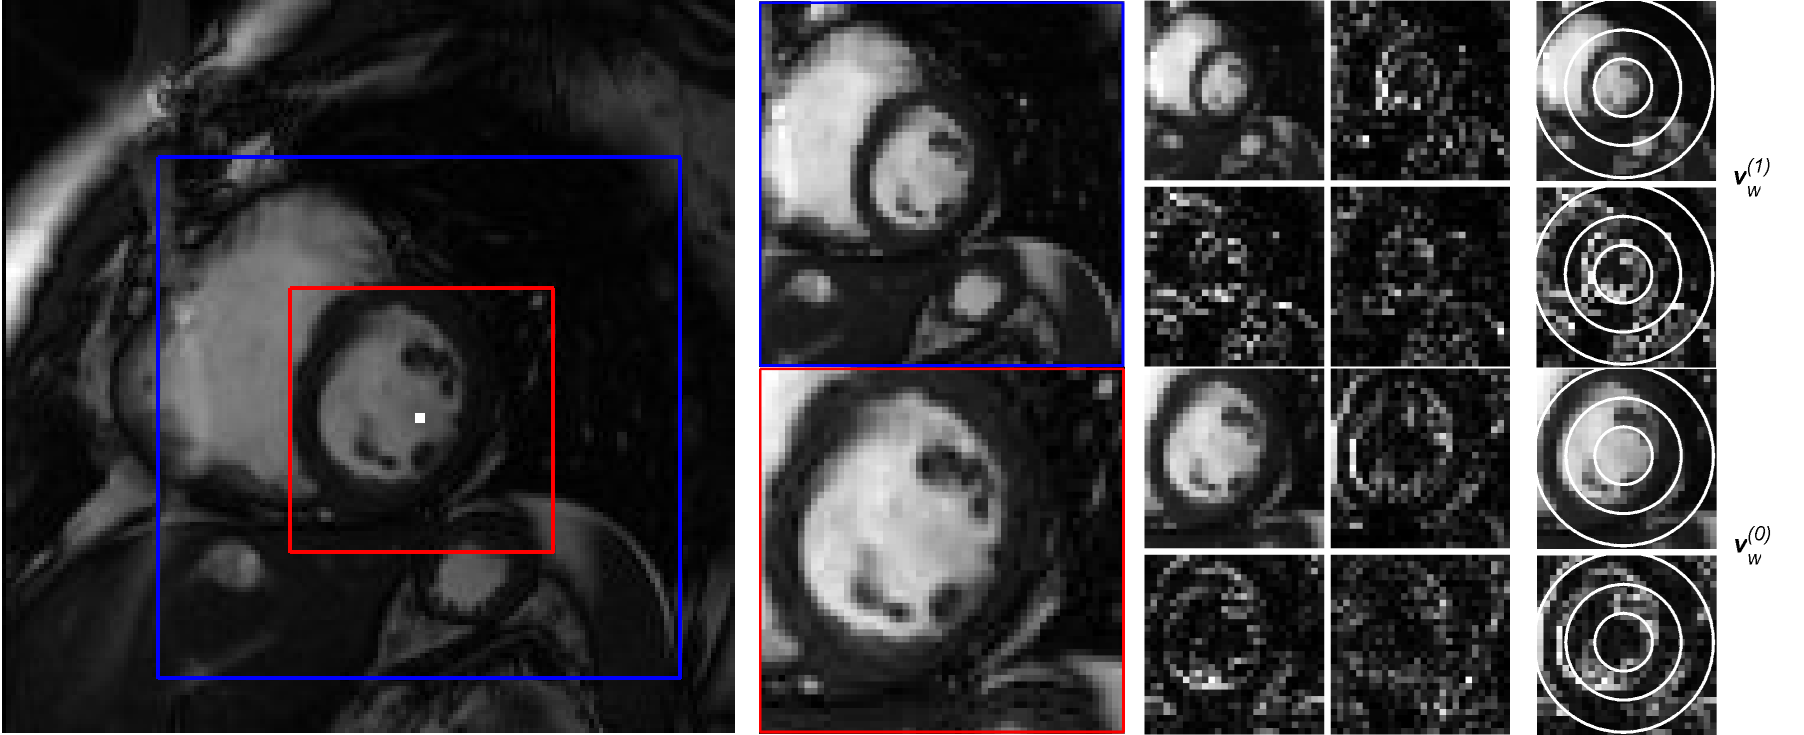
\includegraphics[width=1\textwidth]{images/wav/wav_const}
	   
	   \end{center}  
     \caption{
\em \small Two dimensional illustration of the construction of the wavelet attribute vectors in a multiresolution framework. (a) Input image: the rectangles refer to the sliding windows centered at the current voxel; the large neighborhood corresponds to the relatively low resolution, and the smaller neighborhood to the relatively higher resolution. (b) the image data inside the sliding windows; top: the down-sampled image inside the large window (low-resolution image); bottom: the image inside the small window (high-resolution image). (c) Wavelet decompositions of the images shown in (b); (d) Radial profiling is used to construct the attribute vectors at different resolutions, $\bv _w^{(0)}$ and $\bv _w^{(1)}$, and the wavelet attribute vector is $\bv _w = [\lambda'_0\bv _w^{(0)} , \lambda'_1\bv _w^{(1)}] $
}
     \label{fig:wav_const}
\end{figure}

\subsection{Wavelet attribute vector similarity function}
\label {sec:attribSim}

The similarity between two wavelet attribute vectors $\bA$ and $\bB$ is given by the sum over all resolutions of the angle between the wavelet attributes. We can write this as,
\[
 \varphi(\bA, \bB) = \sum_{r} \eta_r \frac{\left\langle \ba_r, \bb_r\right\rangle}
                                                                  {\left\|\ba_r\right\|\left\|\bb_r\right\|}
\]
where, $\eta_r$ is the weight applied to the attribute vector $\bw_r$ at a given resolution $r$.

\begin{figure}
\begin{center}
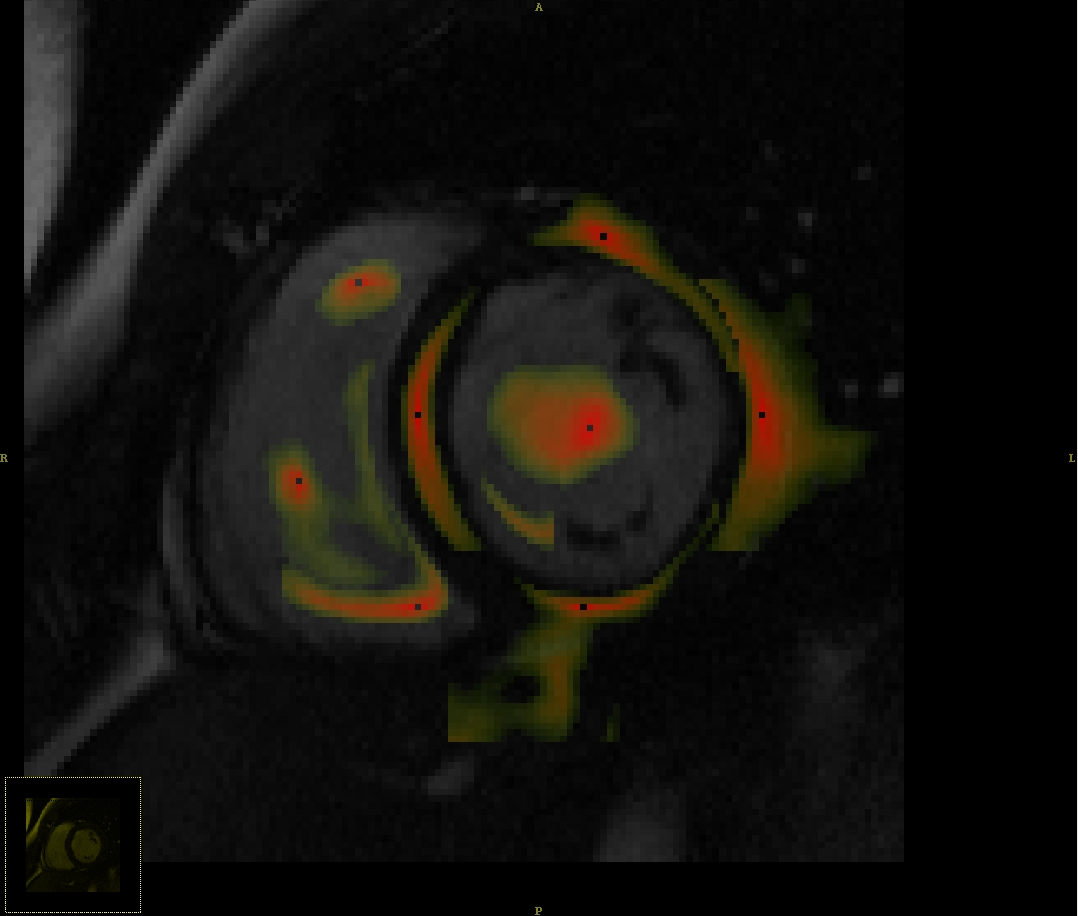
\includegraphics[scale=0.25]{images/wav_local.png} 
\caption{\em \small Wavelet-based attribute vector similarity. The matchmaps, or the similarity in the neighborhood of select points are shown.}
\label{wav-sim}
\end{center}  
\end{figure} 

The effectiveness of the wavelet attribute in capturing the uniqueness of a given voxel can be seen in Figure \ref{wav-sim}. We evaluate the similarity of the attribute vector with the voxels in its neighborhood. As can be seen the attribute vectors are able to localize the voxel effectively. The neighboring voxels show high similarity to the given voxel. The similarity drops as we move away from the voxel. Another thing to notice is that the similarity also drops as we cross over to the blood from the myocardium and vice-versa. Thus the wavelet attribute vectors effectively capture the local and global features of a given voxel. One problem with the wavelet attribute that can be seen in Figure \ref{wav-sim} is that we seem to get \textit{reflections} about blood-myocardium boundaries. This happens to a large part because the wavelet attributes calculated by \cite{wav} are rotation invariant. For cardiac motion estimation it is actually preferable not to have rotation invariant attributes. This will be done in the future.


\begin{figure}
\begin{center}
\subfigure[Original Frame on which the points were selected, with the points shown in blue.]{
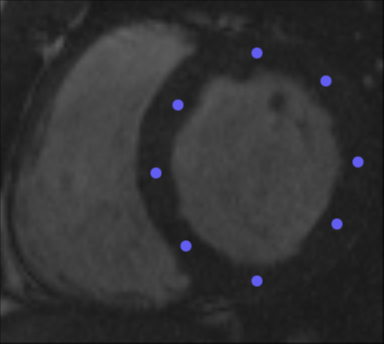
\includegraphics[width=.30\textwidth]{images/frame-01}} 
\hspace{.15in}
\subfigure[The Target Frame, showing the original points in blue. The best correspondence is shown in yellow]{
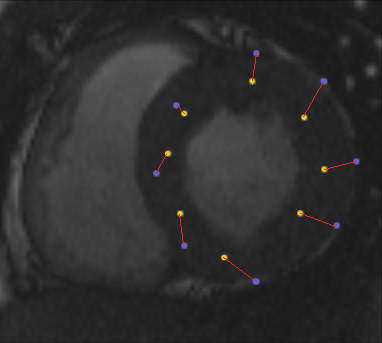
\includegraphics[width=.30\textwidth]{images/frame-10}}
\caption{\em \small Wavelet-based attribute vectors for evaluating deformations within the same subject.}
\label{wav-twist}
\end{center}  
\end{figure}

%\begin{figure}
%\begin{center}
%\subfigure[Original Frame on which the points were selected, with the points shown in blue.]{
%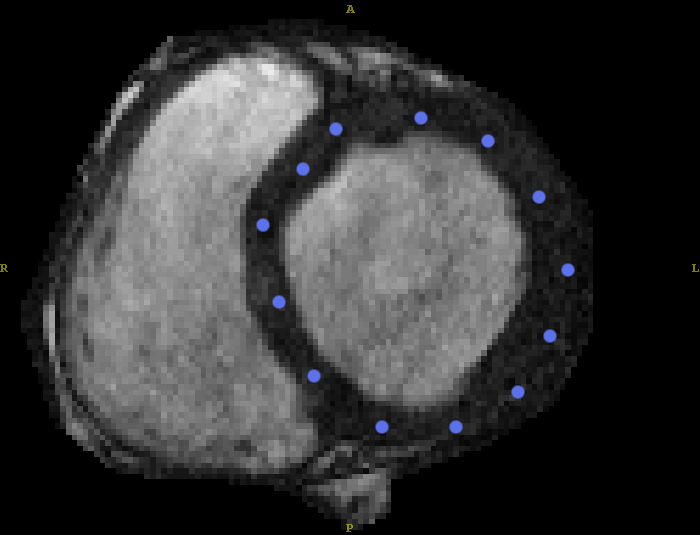
\includegraphics[width=.30\textwidth]{images/wav-t1-06-03}} 
%\hspace{.1in}
%\subfigure[Slice - 1, on the Target Frame. As can be seen some points have moved out of the original plane. This happens because of twisting during the cardiac cycle.]{
%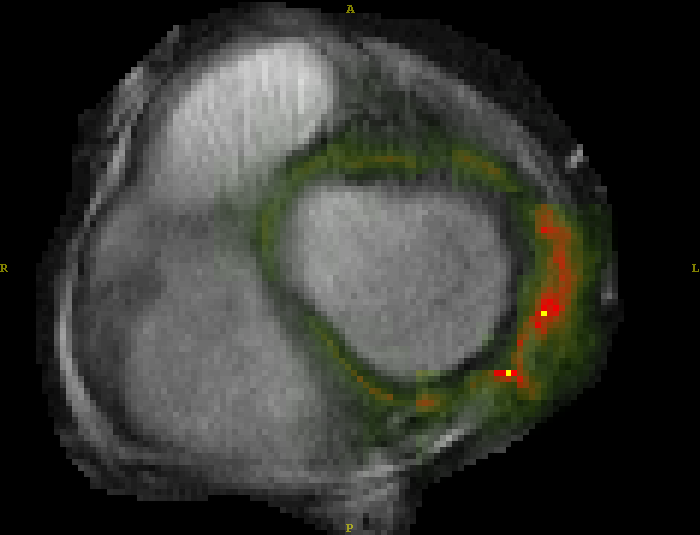
\includegraphics[width=.30\textwidth]{images/wav-t1-06-02}}
%\hspace{.1in}
%\subfigure[Original slice on the Target Frame, showing the matchmap and the original points in blue. The best correspondence is shown in yellow]{
%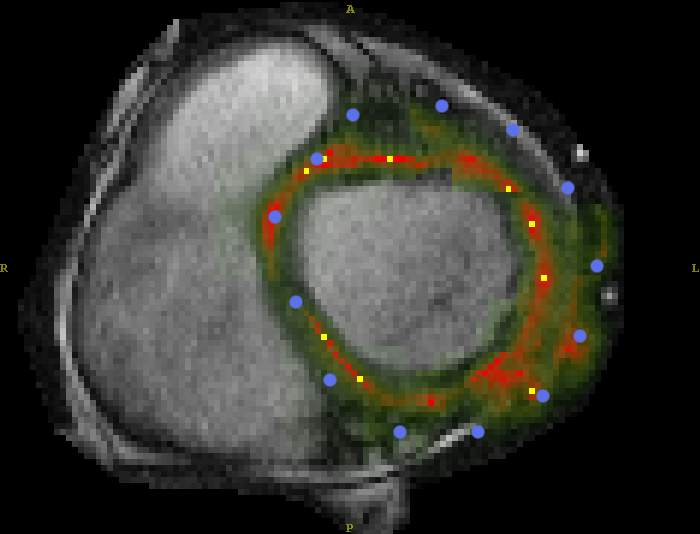
\includegraphics[width=.30\textwidth]{images/wav-t1-06-01}}
%\caption{Wavelet-based attribute vectors for evaluating deformations within the same subject.}
%\label{wav-twist}
%\end{center}  
%\end{figure} 

\subsection{Selecting the best correspondence point}

Instead of using inverse consistency for determining the best match for a given voxel as done in \cite{wav}, we instead use an alternate strategy. We compute the similarity $\varphi$ of the point $p$ defined on the end-diastole frame, $I_0$, to points within a search radius, $r$, in the image $I_t$. We test the similarity between the point $\bp$ on $I_0$ and the neighboring points, $\bp + \bepsilon$, on $I_t$, where $\|\bepsilon_i\| \le r$. The points in $I_t$ together with their similarity values to the point $\bp$ define a {\em matchmap} \cite{guest01}. This can be seen in Figure \ref{wav-sim}. We select the best corresponding point by integrating over the matchmap. We want to weight the points by the similarity, therefore we assign weights to the points based on their similarity,
\[
	\gamma_i = \varphi(\bW_{I_0}(\bp), \bW_{I_t}((\bp + \bepsilon_i)))
	%\gamma_i = \frac {\varphi(\bW_{I_0}(\bp), \bW_{I_t}((\bp + \bepsilon_i)))}{1 + |\bepsilon_i|^b},~~~~~~~~~b\ge2,
\]
where, $\bW_I(\bx)$ is the wavelet attribute vector at point $\bx$ on image $I$, and $\bp + \bepsilon_i$ is a point within the search radius.
%where, $W_I(\vec{x})$ is the wavelet attribute vector at point $\vec{x}$ on image $I$, and $\vec{\epsilon}_i$ is the perturbation applied to the point $\vec{p}$ within the search radius, and $b$ is a constant. 
%We use a value of 2.0 for $b$, so that points that are far away can still influence of the corresponding point if they match well. 
Using this, the best corresponding point, $\bx_c$, is given by the weighted mean of the points, where the weights are $\gamma_i$ defined above, 

\[
\bx_c = \frac {\sum \gamma_i (\bp + \bepsilon_i) } { \sum \gamma_i }
\]
the summation being evaluated over a neighborhood of the point $\bp$.

This makes the correspondence detection more robust and also imposes smoothness constraints. The results from this formulation can be seen in Figure \ref{wav-twist}. The best correspondence points are shown in yellow. These typically lie in another plane and are thus shown in two frames, one with the original points in blue and the other with the detected points. The twist within the myocardium is clearly visible. These results make us believe that along with smoothness constraints, the wavelet attributes along with the weighted correspondence estimation are best suited to extract cardiac motion fields.

We also observe that the wavelet attribute vectors are very effective in detecting correspondence across subjects. This can be seen in Figure \ref{fig:wav-sub}. Here the points in the template image are shown in blue. The detected corresponding points are shown in yellow. As we can see, the attribute vectors are able to identify the corresponding points both the in the end-diastole image, i.e., the one with no deformation and the end-systole image, the one with maximum deformation, Figure \ref{fig:wav-sub2}. Thus we see that the wavelet-based attribute vectors are both robust and accurate across time and across subjects. Also, the similarity computation between the attribute vectors, described in Section \ref{sec:attribSim} is very fast and thus makes the actual registration very efficient. 

\begin{figure}
     \centering
     \subfigure[The template image on which the points are selected. Shown here in blue.]{
          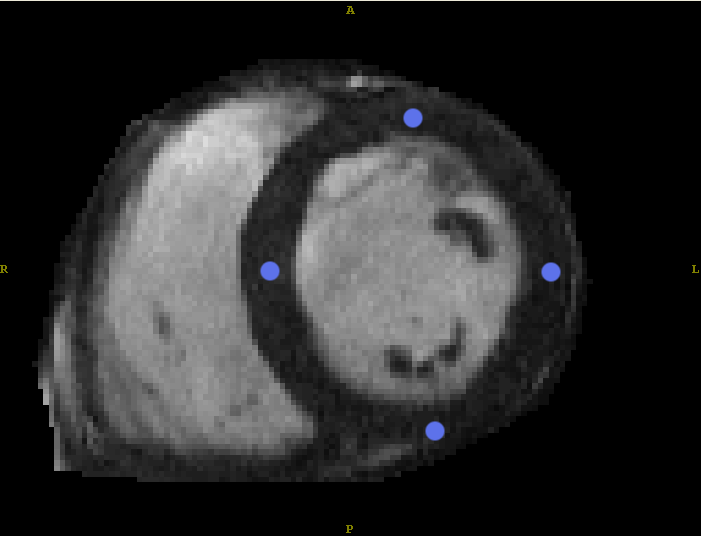
\includegraphics[width=.30\textwidth]{images/wav-p1-01-t1}
          \label{fig:wav-sub-tem}}     
     \hspace{.1in}     
     \subfigure[The subject image, same frame, adjacent slice. The best correspondence is shown in yellow.]{
          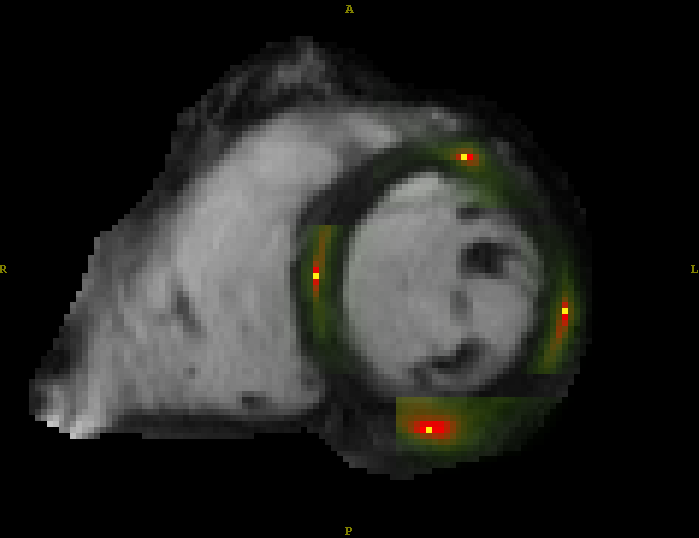
\includegraphics[width=.3\textwidth]{images/wav-p1-01-y}}
     %%\hspace{.05in}
     \hspace{.1in}
     \subfigure[The subject image, same frame, same slice. We show the selected points in the template space, overlaid in blue.]{
          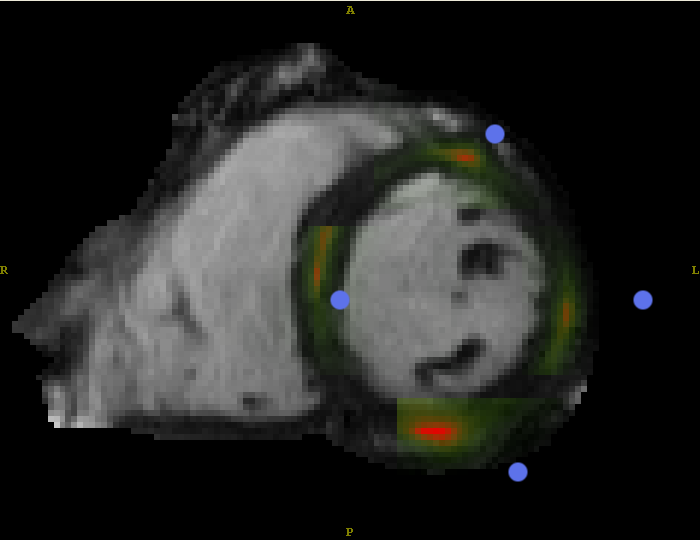
\includegraphics[width=.3\textwidth]{images/wav-p1-01-b}}
     \caption{\em \small Attribute similarity across different Subjects}     
     \label{fig:wav-sub}
\end{figure}

\begin{figure}
     \centering
     \subfigure[The subject image shown further along cardiac cycle, slice - 3. One of the points is detected on this slice]{
          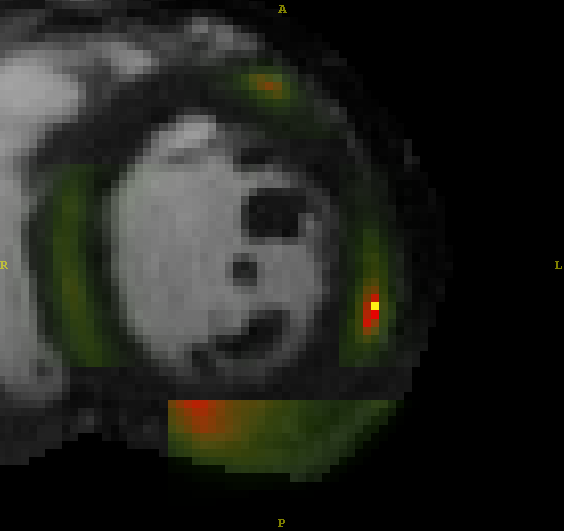
\includegraphics[width=.2\textwidth]{images/wav-p1-06-01}}
     %%\hspace{.05in}
     \hspace{.1in}
     \subfigure[The subject image shown further along cardiac cycle, slice - 2. One of the points is detected on this slice]{
          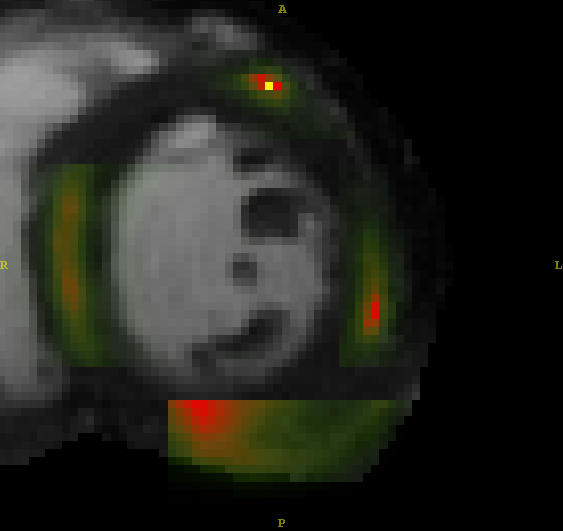
\includegraphics[width=.2\textwidth]{images/wav-p1-06-02}}
     %%\hspace{.05in}
     \hspace{.1in}
     \subfigure[The subject image shown further along cardiac cycle, slice - 1. Two of the points are detected on this slice]{
           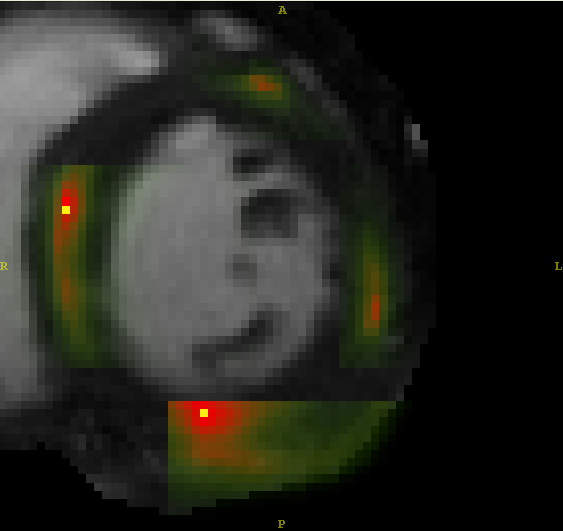
\includegraphics[width=.2\textwidth]{images/wav-p1-06-03}}
     \hspace{.1in}      
     \subfigure[The subject image shown further along cardiac cycle, the same slice. The points picked in the template space are shown in blue.]{
           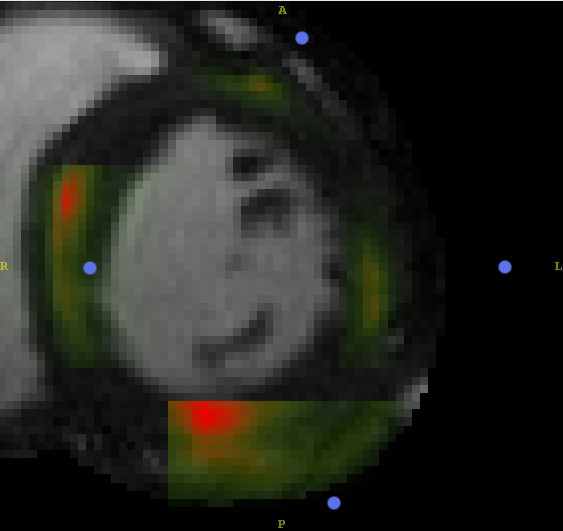
\includegraphics[width=.2\textwidth]{images/wav-p1-06-04}}
     \caption{\em \small Attribute similarity across different Subjects and different time frames}
     \label{fig:wav-sub2}
\end{figure}

\subsection {Distinctiveness of attribute vectors}
\label{sec:wav-distinctive}
In order to be able to pick focus points to drive the registration, we need to be able to select attribute vectors based on how distinctive they are. Doing this will allow us to robustly perform the registration in a fast hierarchical manner. This also allows us to select focus points automatically based on the distinctiveness of the attribute vectors. Also we weight the similarity of the points, during the energy function evaluation by the distinctiveness of the point. If we perturb each point in the end-diastole image $I_0$ and evaluate the best correspondence point for each of these points, we will get a scatter of best correspondence points. The distribution of this scatter of points provides information about the robustness of each match to image $I_t$ \cite{guest01}. 

\begin{figure}
\begin{center}
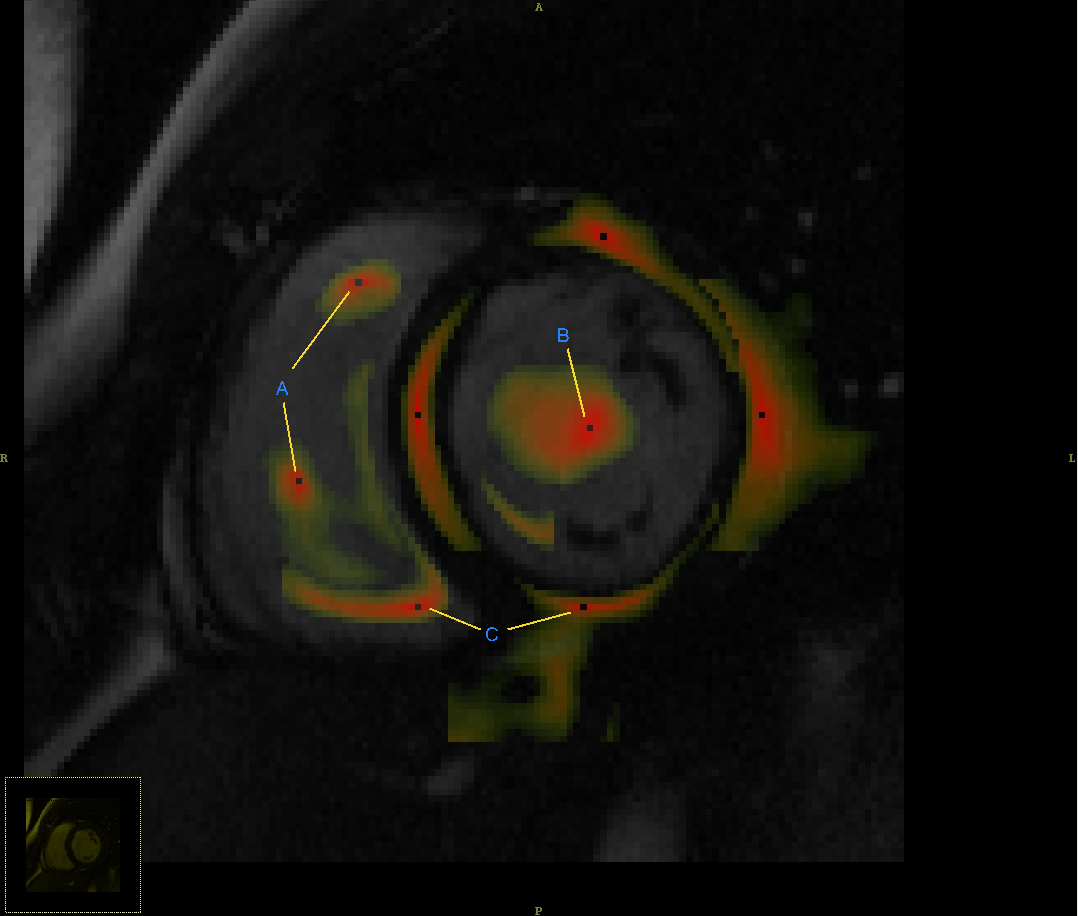
\includegraphics[scale=0.25]{images/dist_explain.png} 
\caption{\em \small Different kinds of matchmaps. Points A are points with high distinctiveness as their spread is small. Point B has low distinctiveness as it has a large spread. Points C also have relatively low distinctiveness, since the spread is large along one of the axes}
\label{dist-exp}
\end{center}  
\end{figure}

To understand how we define the distinctiveness of a given voxel based on the wavelet attributes, consider Figure \ref{dist-exp}. We can see that different voxels produce different scatters based on the local and global characteristics of the underlying image. Although we get sharp peaks for all three types, (A,B, and C), we observe that for {\bf A} the scatter is localized and the spread is uniform and small in all directions. In case of {\bf B}, the spread is more or less uniform but it is large. The distinctiveness of such points is low, because there are a lot of points which are relatively far from the actual point that have sufficiently high similarity. The confidence in the similarity of such points is lower since we could be sufficiently far from the best point (in mm) and still have a fairly high similarity. Such points can increase the error in registration, and should therefore be avoided. The third set of points, {\bf C} is also not very distinct, because although they are heavily localized in one direction, there is a very large spread along the principal axes. Again such points can increase the error in registration and should be assigned low {\em distinctiveness}. 

\begin{figure}
\centering
     \subfigure[Distinct point that has low spatial spread and is static, i.e., has no motion]{
          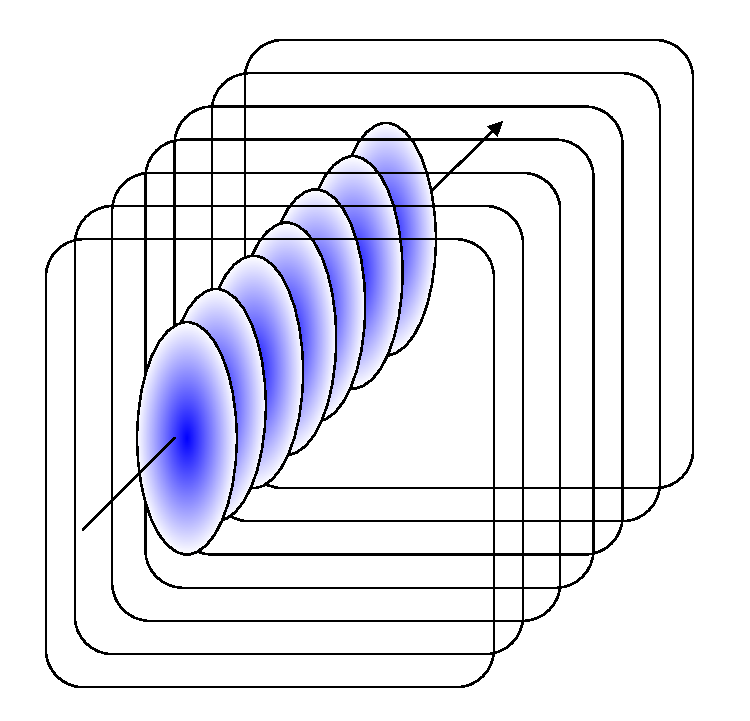
\includegraphics[height=.27\textwidth]{images/dist-a}
          \label{fig:dist-a}
          }
     \hspace{.1in}     
     %%\hspace{.05in}
     \subfigure[Distinct point, that has low spatial spread and has temporally smooth motion]{
          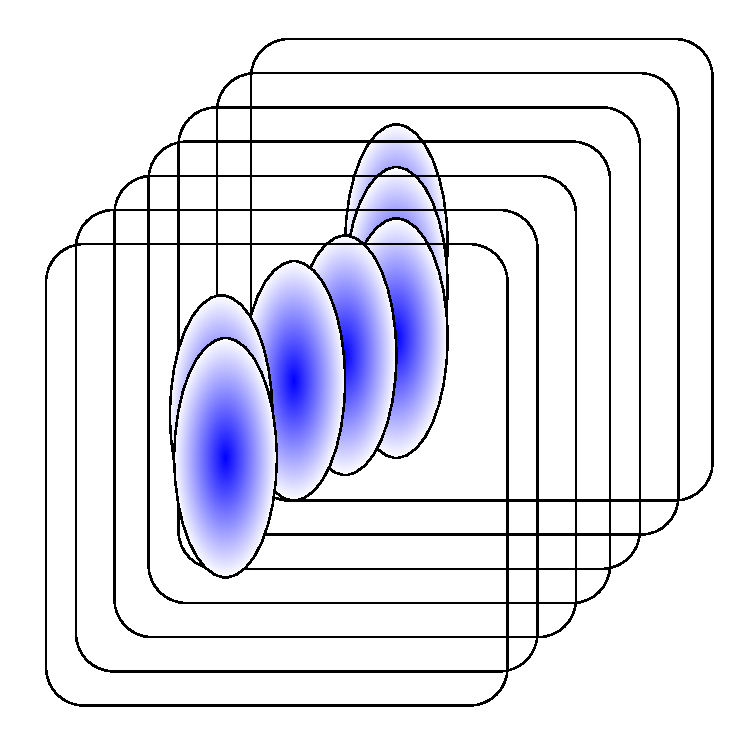
\includegraphics[width=.27\textwidth]{images/dist-b}
          \label{fig:dist-b}
          }
     \hspace{.1in}     
     \subfigure[Non distinct point that has large spatial spread and haphazard temporal motion]{
          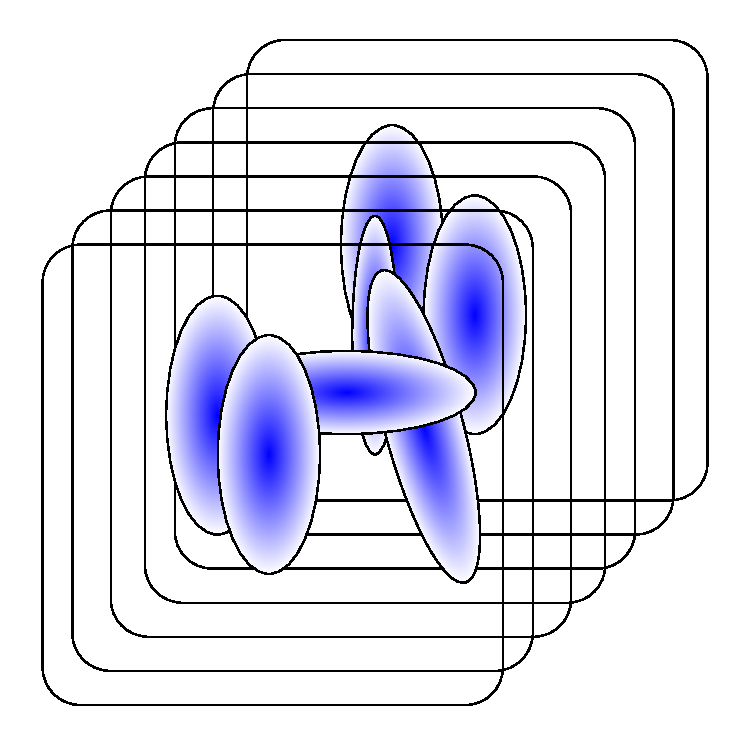
\includegraphics[width=.27\textwidth]{images/dist-c}
          \label{fig:dist-c}     
          }
     \caption{Distinctiveness of a point over a sequence}     
     \label{fig:dist-seq}
\end{figure} 

The situation is a bit different when we consider a sequence of such images, and their matchmaps over time. Some of the common cases that can occur are shown in Figure \ref{fig:dist-seq}. One common case is of points that are localized spatially and temporally consistent, as shown in Figure \ref{fig:dist-a}. These kinds of points typically can be found outside the pericardium, i.e., tissues and bones which do not move much during the cardiac cycle. Figure \ref{fig:dist-b} shows the case that is ideally preferred for points within the myocardium. These are points whose spatial spread is low, and temporally smooth motion can be observed. Figure \ref{fig:dist-c} shows the case of a point whose matchmaps are scattered across slices, and the confidence in estimating the location of this point across slices is low. Therefore, we assign a low distinctiveness to such points. This amounts to a distinctive point having a large spread along the time axis, and much smaller localized spreads along the spatial dimensions.

We extend this to the 4D case, where the only difference is that we wish for the spread along the time axis to be large, and the other three to be small. In order to compute the distinctiveness of the selected point, we calculate the eigenvalues and eigenvectors from the moment of inertia matrix obtained from the 4D matchmap. The 4D moment of inertia matrix of the matchmap is defined as,

\begin{equation}
\label{eq:moi}
I = \sum_i \gamma_i \left[ 
\begin{array}{cccc}
	y_i^2+z_i^2+t_i^2 & -x_iy_i & -x_iz_i & -x_it_i \\
	-x_iy_i & x_i^2+z_i^2+t_i^2 &  -y_iz_i & -y_it_i \\
	-x_iz_i & -y_iz_i & x_i^2+y_i^2+t_i^2 &  -z_it_i \\
	-x_it_i & -y_it_i  &  -z_it_i & x_i^2+y_i^2+z_i^2 
\end{array}
\right]
\end{equation}

We prefer points whose similarity matchmaps are spatially localized and compact. They should also be temporally smooth. This means that the 4D scatter in a 4D neighborhood for distinct points should be a 4D cylinder. We therefore compute the eigenvalues of the moment of inertia matrix, defined in (\ref{eq:moi}), and assign high distinctiveness to all points which have one large eigenvalue and three small eigenvalues. Here we are basically trying to keep the spatial spread low. Because of the way the 4D matchmap is evaluated, the temporal spread will be large. For points which do not move much, the principal eigenvector will be aligned with the {\em time} axis. Correspondingly as the motion of the point in question increases, the angle between the principal eigenvector and the {\em time} axis will increase. Since we wish to give more importance to points with large motion. Therefore we scale the distinctiveness factor by the angle between the principal eigenvector and the {\em time} axis.

%In the 3D case, there are three eigenvalues and eigenvectors. If all the eigenvalues are small, the tentative corresponding points are clustered near a point. If the second and third eigenvalues are small, the tentative corresponding points are scattered along a line; and if only the third eigenvalue is small, they are scattered in a plane. When all the eigenvalues are large, the tentative corresponding points are widely scattered. We use the values of these eigenvalues as an estimate of how reliable a given point is for determining correspondence. When the points are widely scattered, i.e., the case when all three eigenvalues are large, we place low confidence on the reliability of that point. Conversely, the best points are those which are clustered about a point, i.e., those that have all small eigenvalues. 

\begin{figure}
	\centering
	  \subfigure[Distinctiveness calculated over the whole image. We can see that it is low along the peripheries and also within the blood pool.]{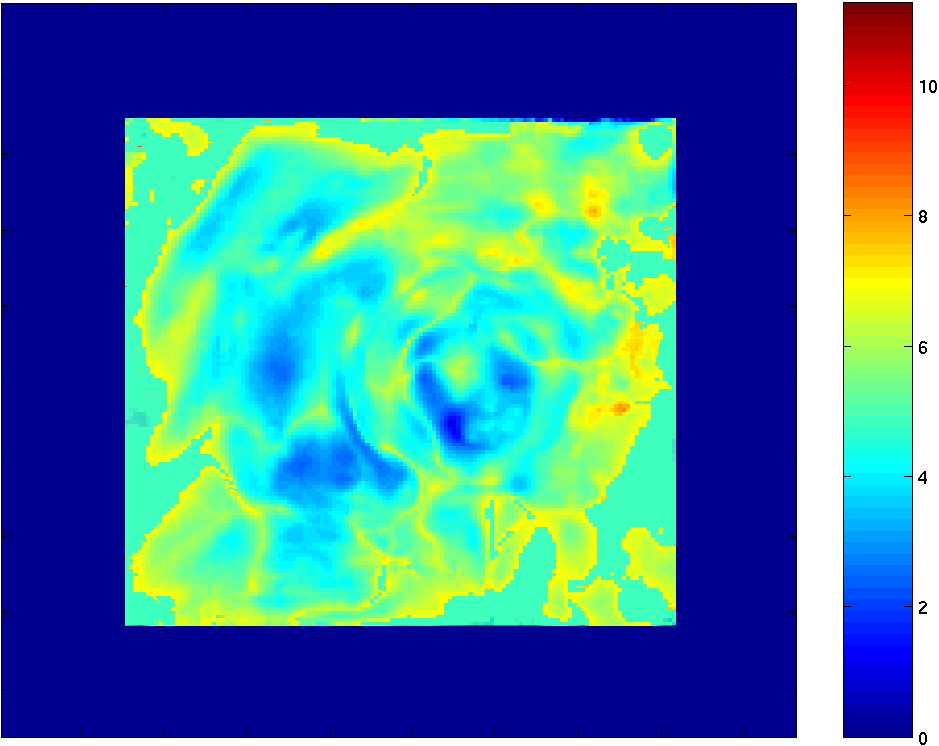
\includegraphics[height=.25\textheight]{images/hari-dist2}}
	  \hspace{.15in}
		\subfigure[Overlay of the distinctiveness to show the distinctiveness on the myocardial region]{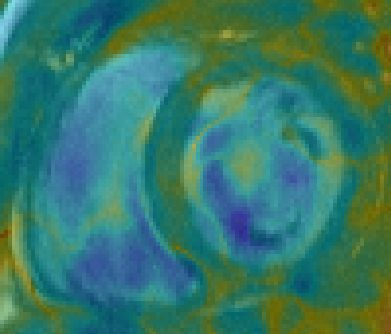
\includegraphics[height=.25\textheight]{images/distinctiveness}}
	\caption{The distinctiveness of voxels, based on the wavelet attribute vectors}
	\label{fig:distinctiveness}
\end{figure}

The distinctiveness of the voxels as computed by this method is shown in Figure \ref{fig:distinctiveness}. As can be seen this is proportional to both the level of structural as well as motion relation features, which is what we are trying to extract. We can use this these {\em distinctiveness} values to compute a multiresolution set of {\em focus} points. 


\section{Estimating the Cardiac Motion Field}
\label{sec:CarMot}

Cardiac motion estimation is the problem of determining a transformation that captures the motion of every point in the myocardium over the cardiac cycle. If we can register 3D images acquired at different phases of the cardiac cycle to each other, then we have an estimate of cardiac motion. Thus we can formulate the problem as one of being able to track (detect correspondence) of a small set of points on the myocardium over the entire cardiac cycle. 

These points are the ones whose motion can be estimated most reliably. These are selected based on their distinctiveness, Section \ref{sec:wav-distinctive}. This makes the registration more robust as it is not affected by points with low distinctiveness, i.e., those points whose correspondence cannot be determined with high confidence. Another advantage of using the {\em focus} points is that it makes the similarity computation faster. It also reduces the dimensionality of the cost function, making the optimization more robust and faster. All these factors together make the current formulation robust and fast. 
%We solve only for the correspondence of a small set of {\em focus} points because we want the estimation process to be fast. 
Since the myocardium moves as one connected object and the motion is smooth, we can interpolate the transformation at the focus points to get the transformation over the whole myocardium. 

The problem of motion estimation from cardiac cine images is ill posed, and relying solely on image similarity, even with very accurate similarity measures is not sufficient to capture the true motion of the heart. Current cardiac motion estimation methods rely on image similarity measure to drive the motion estimation, and typically incorporate a regularizer to smooth the deformation field. We propose to instead maximize the similarity between the wavelet attributes, subject to the motion estimate constrained by a mechanical model of the heart, which has been discussed in Section \ref{sec:model}.

The result of a 4D scan of a beating heart is a periodic sequence of $N$ 3-$D$ images,
\[
I(\bx,t) = \{I_t(\bx), 0\le t < N\}
\] 
where $I_0$ is the end-diastolic image. We define the motion field as the transformation $\bchi ( \bx, t )$ defined over the image space. The transformation maps a point $\bx$ in the end-diastole frame $I_0$ of the image to its corresponding point in frame $I_t$ at time $t$. This is illustrated in Figure \ref{fig:motion}. The displacement field $\bU( \bx, t )$  defines the mapping from the coordinate system of the end-diastole image $I_0$ to the image at time $t$, $I_t$. The transformation and the displacement are related as, $\bchi( \bx ,t ) = \bx + \bU( \bx, t)$.

\begin{figure}
\begin{center}
\includegraphics[width=.75\textwidth]{images/motion-est} 
\caption{Formulation of the cardiac motion extraction problem.}
\label{fig:motion}
\end{center}  
\end{figure} 

A sparse set of focus points $\bp \in \Omega$ needs to be defined on the end-diastole image $I_0$. This can either be done manually, by the user, or using some feature extraction policy. Automatic focus point selection as described in Section \ref{sec:wav-distinctive} is used to select focus points at different resolutions to be used with the multiresolution approach. These points are tracked through the entire sequence $I(\bx, t)$ in order to determine the correspondences and estimate the motion field $\bchi ( \bx, t )$. We solve an energy minimization problem where we solve for the deformation vectors at each of these points at each time frame.

To allow the registration algorithm to focus on different sets of points adaptively during different stages of image registration, each point should have it's own energy term and the overall energy function should be a weighted summation of energy terms of all the points. Therefore, by hierarchically assigning weights, $\eta ( \bx)$,  according to the distinctiveness of the attribute vectors (Section \ref{sec:wav-distinctive}), we can focus on the most suitable points to actively drive the image registration. This increases the reliability of the motion estimation as it is not affected by the similarity estimates of unreliable points. The other benefit is that of improved speed of the motion estimation. If we were to solve for the displacement at every grid point on the image, then the dimensionality of the cost function that we are minimizing will be extremely high. Also the cost function evaluation would be much more expensive. Solving for the displacements at only the focus points, allows us to reduce the dimensionality of the problem and also makes the cost function evaluation much faster. Thus the procedure approximates a very high-dimensional cost function (equal to the number of points in the image sequence) by a significantly lower-dimensional cost function of only the active points. This makes the minimization process much faster and also less susceptible to getting trapped in local minima, as it is a function of the focus points for which we can find relatively unambiguous matches. The method also performs much better than a simple subsampling of the original grid to reduce dimensionality, since in essence we create an adaptive grid that is dense in areas with more distinctive features and sparse in areas which are relatively static or where the confidence in the similarity is low.

We present the motion problem as a non-linear pde constrained optimization problem. Most systems can be thought of as having certain control parameters $g$, which directly or indirectly affect the process' state $\phi$. An optimization problem can be thought of as one of finding controls $g$ and states $\phi$ such that a cost functional $\mathcal{C}(\phi, g)$ is minimized subject to $\mathcal{F}(\phi, g)=0$.  Here the cost functional $\mathcal{C}(\phi, g)$ is a measure of the how close the current state is to the desired one. $\mathcal{F}(\phi, g)=0$ is a constraint on the relationship between the states and the controls. For the problem of cardiac motion estimation, we solve for the forces $\tau$ in the myocardial fibers and obtain the states $\bu$, the displacements produced as a result of these forces. The constraint, $\mathcal{F}(\bu, \tau)=0$ is the mechanical model described in Section \ref{sec:model},

\[
\mathcal{F}(\bu, \tau) = \rho_0\dudtsq - \mbox{Div}(\lambda \ln\mathcal{J}\bF^{-T} + \mu(\bF -\bF^{-T})) - \sigma\bF\bn = 0 \mbox{~~~~in~} \Omega
\]

The cost functional that we minimize, is the wavelet similarity term discussed earlier in Section \ref{sec:attribSim}. The similarity is computed between the wavelet attribute vectors at the point $\bchi ( \bx, t )$, $\bW ( \bchi ( \bx, t ) )$ and at the point $\bchi ( \bx, t + 1 )$, $\bW ( \bchi ( \bx, t + 1 ) )$. The Energy function for point similarity, summed over all the focus points, $\bp$, over all time frames is,
\begin{equation} 
\label{eq:wav-sim}
   \mathcal{C}(\bu, \tau) = \sum_{t = 0}^{N - 1} \sum_{\bx \in \{\bp \}} \eta (
     \bx) \left( \sum_{\bz \in n ( \bx, 0 )} \varphi \left(
     \bW ( \bchi ( \bz, t ) ), \bW ( \bchi ( \bz, t + 1 ) ) \right)
     \right) 
\end{equation}

The importance of each point $\bx$, in the registration is determined by the corresponding parameter $\eta (\bx )$, which is designed to be proportional to the distinctiveness of the point's wavelet-based attribute vector. The match for each point $(\bx, t)$ is evaluated in it's 3-$D$ neighborhood $n ( \bx, 0 )$, by integrating the similarity measure between the attribute vector $\bW( \bchi ( \bz, t ) )$  of every neighboring point $( \bz, t )$ and the attribute vector $\bW ( \bchi ( \bz, t+1 ) )$ of the corresponding point in the adjacent time frame of the sequence. The is equivalent to matching image patches or volumes between the two images because of the following two reasons,

\begin{itemize}
	\item The attribute vector is calculated in a local neighborhood and therefore represents information in the neighborhood of the voxel in question.
	\item We sum over the similarities in the neighborhood of $\bx$ when evaluating the wavelet similarity term (\ref{eq:wav-sim}).
\end{itemize}

The size of the neighborhood is large initially and decreases gradually with the progress of the deformation, thereby increasing robustness and accuracy of the motion estimation. As the neighborhood size is decreased we also change the weights for the multi-resolution attribute vectors similarity, increasing the weights for the fine features and decreasing the weights on the global features. This is equivalent to reducing the size of the image patches being matched as we move to the higher resolutions.

The optimization algorithm can be solved by using the following algorithm,

%\begin{algorithm}
%\caption{Cardiac Motion Estimation Algorithm} \label{MotAlg}
%\begin{algorithmic} [1]
%\STATE i=0, Initial guess for forces, $\tau^{(0)}$
%\WHILE {solution not converged}
%\STATE \textbf{solve} $\mathcal{F}(\bu^{(i)}, \tau^{(i)})=0$ to obtain displacements; \COMMENT{The mechanical model}
%	\STATE \textbf{compute} the gradient of the functional $\frac{\partial \mathcal{C}}{\partial \tau}(\bu^{(i)}, \tau^{(i)})$;
%	\STATE \textbf{compute} the step $\delta \tau^{(i)}$
%	\STATE \textbf{set} $\tau^{(i+1)} = \tau^{(i)} + \delta \tau^{(i)}$
%\ENDWHILE
%\end{algorithmic}
%\end{algorithm}


\section {Periodicity Constraint}
Since the image sequence is periodic, i.e.,  the first image $I_0$ and the last image $I_{N-1}$ are also temporal neighbors, as shown in Figure \ref{fig:motion}. We impose a hard constraint on the deformations to return a point $\bx$ to itself after the full cardiac cycle, i.e., $( \bx, 0 ) = \chi ( \bx, N-1 )$. This is done by ensuring that during each step of the minimization,

\begin{equation}
\sum_{\bx \in \{ \bp \}} \| \bchi ( \bx, N-1 ) - ( \bx, 0 ) \| = 0 
\end{equation}s